\subsubsection{Aufsetzen von QtCreator}

QtCreator ist eine integrierte Entwicklungsumgebung, die von Qt selbst zur
Verfügung gestellt wird und somit alle Features von Qt (qml, Widget-Designer, ...)
nativ unterstützt. Da die IDE auch C++-Programmierung unterstützt, eignet sie
sich als Allrounder-IDE für dieses Projekt.\\

Im Folgenden wird das Aufsetzen von QtCreator und erste Schritte danach für
\textbf{Ubuntu 16.10} beschrieben:\\

\textbf{QtCreator installieren}\\
Über den Paketmanager:
\begin{lstlisting}
apt install qtcreator
\end{lstlisting}

\textbf{Repository klonen}\\
Siehe \autoref{dev-report-cmake-build}. Endet die Ausführung von cmake in einem
Fehler (``Could not find a package configuration file provided by Qt5Widgets``),
dann ist vermutlich bei der Installation von \texttt{qtdeclarative5-dev} etwas
schiefgegangen.\\

\textbf{In QtCreator CMake-Projekt einrichten}\\
Im Startbildschirm ``Open Project'' und dann die oberste \texttt{CMakeLists.txt}
(die in \texttt{era-gp-sim/CMakeLists.txt}) öffnen.\\ Im Reiter ''Configure
Project'' für das Kit ''Desktop'' -> Details: Nur Debug und Release anhaken und
die Build-Ordner anpassen\footnote{Es bietet sich an, für die IDE einen anderen
Build-Ordner zu verwenden, als für das Bauen über die Konsole. Ein CMake-Projekt
in QtCreator wird mit CodeBlocks erzeugt und erstellt daher leicht andere
Konfigurationsdateien als cmake über die Konsole. Damit beides parallel
nebeneinander betrieben werden kann, sollten die Build-Ordner getrennt werden.}.
Die Auswahl bestätigen.\\ Jetzt sollte das Edit-Tab mit dem Projekt geöffnet
sein. Im unteren Rand unter ''General Messages'' sollte einmal cmake automatisch
aufgerufen worden sein, links oben im ''Projects'' Fenster sollte die Struktur
des Projekts (mit CMakeLists.txt, include, source, tests und third-party) zu
sehen sein.\\ Im Projects-Tab (linker Rand, Schraubenschlüssel) im Reiter
''Build \& Run'' wird jetzt der Build-Prozess konfiguriert. Bei ''Edit build
configuration'' Debug auswählen, dann unter ''Build Steps'' folgendes
verändern:\\
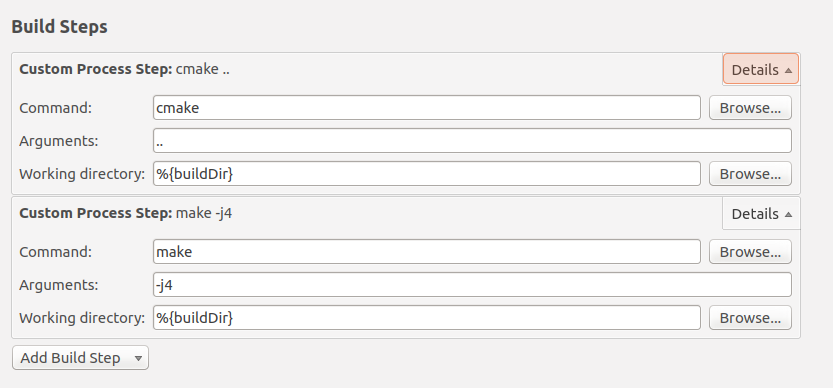
\includegraphics[scale=0.5]{images/setup-qtcreator-buildrun-config.png}\\ Der
Eintrag von cmake Arguments soll dabei der relative Pfad vom eingetragenen
Build-Ordner zum obersten Ordner des Projekts sein. Im Beispiel ist der
Build-Order unter \texttt{era-gp-sim/build\_qtcreator\_debug} angelegt, d.h.
eine Ebene höher liegt der root-Ordner des Projekts. Das \texttt{-j4} Argument
bei \texttt{make} erhöht die Geschwindigkeit beim Bauen, da 4 Jobs gleichzeitig
ausgeführt werden. Zur Run-Konfiguration wechseln
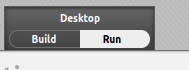
\includegraphics[scale=1.0]{images/setup-qtcreator-run-config} und als ''Working
Directory'' den Build-Ordner eintragen.\\

Nun zurück wechseln und bei ''Edit build configuration'' Release auswählen und
sowohl ''Build Steps'' als auch ''Run'' wie oben verändern.\\

Ins Edit-Tab wechseln und am linken Rand unten beim Monitor von ''Release'' auf
''Debug'' wechseln und dann mit Klick auf den Hammer das Projekt bauen.\\
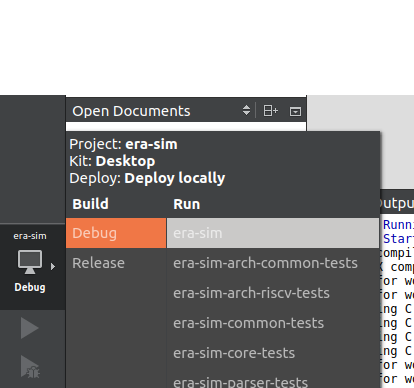
\includegraphics[scale=0.7]{images/setup-qtcreator-change-buildrun-flavor.png}\\
Hier können dann auch später statt ''era-sim'' verschiedene Test-Suits lokal
ausgeführt werden. In der ''Compile Output'' Konsole kann der Fortschritt des
Bauvorgangs überwacht werden.\\


\textbf{Nützliche Einstellungen}\\
\begin{itemize}
	\item File Naming:\\
  Im Menü \texttt{Tools -> Options}, dort in der linken Auswahlliste C++ ->
  Reiter ''File Naming'':\\ Bei Headers Suffix zu hpp ändern.

	\item Lizenz automatisch einfügen:\\

  Im Menü \texttt{Tools -> Options -> C++ -> FileNaming}: Unter ''License
  Template'' kann der Pfad zu einer Textdatei eingegeben werden, deren Inhalt
  dann als Kommentar an den Anfang jeder neu erzeugten Datei platziert wird.

	\item Auto-Formatting (Plugin):\\

  Muss evtl. über \texttt{Help -> About plugins} herunterladen (''Beautifier'').
  Ist dann unter \texttt{Tools -> Options -> Beautifier} zu finden.
  \end{itemize}
\textbf{Erste Schritte}\\
\begin{itemize}
	\item Neue Datei erstellen:\\
	\texttt{File -> New File or Project}
	\item Aktuelle Datei formatieren:\\
	\texttt{Tools -> Beautifier -> ClangFormat -> Format Current File}
\end{itemize}
